%% $Id$
%%
%% Kapitel 2 - Die Oberflaeche
%%

\chapter{Benutzerinterface}

\section{"Uberblick} 

Das Men"u {\bf Datei} enth"alt Funktionen zur Dateiverwaltung, wie
beispielsweise "Offnen und Schlie"sen. Weiterhin kann unter {\bf
Zuletzt benutzt} schnell auf die aktuellsten Dateien zugegriffen
werden. Unter {\bf Bearbeiten} sind Editorfunktionen enthalten. Die
einzelnen Komponenten werden in Kapitel~\ref{Qelltexteditor}
und~\ref{Beweiswerkzeuge} genauer betrachtet. Mit {\bf
Einstellungen...} kann die
Einf"arbung von Schl"usselworten im
Quelltexteditor~\ref{Qelltexteditor} und andere Farben eingestellt werden. Das Men"u {\bf Beweis}
enth"alt die einzelnen Beweiswerkzeuge und dient dazu zwischen dem
{\bf Beginner} und {\bf Fortgeschrittener} Modus zu wechseln. Diese
Modi beeinflussen die bei den Beweisschritten zur Verf"ugung
stehenden Regeln und beeinflusst die Ansicht der verschiedenen Modi. 

\section {Quelltexteditor}
\label{Qelltexteditor} Jede ge"offnete Datei wird in einem Tab
angezeigt, der den Dateinamen angibt. Zwischen den Tabs kann mit
{\bf Strg + Bildhoch/Bildrunter} und {\bf Alt + Rechts/Links}
gewechselt werden.

Jeder Datei ist eine Sprache fest zugeordnet. M"ochte man einen
Ausdruck in einer anderen Sprache beweisen, so kann man hierf"ur
einen neuen Editor "offnen und der Ausdruck kopieren. Alternativ
kann auch die Dateiendung einer gespeicherten Datei ge"andert
werden. Ist ein eingegebener Ausdruck fehlerhaft, so wird dies links
von der betroffenen Zeile durch ein Error-Icon markiert. Zus"atzlich 
wird der fehlerhafte Teil rot unterstrichen. 

Bewegt man den Mauszeiger "uber den markierten Text oder das Error-Icon,
so erscheint ein Tooltip, der den Fehler genauer beschreibt. Ein Klick
auf das Error-Icon bewirkt, dass der fehlerhafte Text markiert wird. Wird
nun noch einmal auf das Error-Icon geklickt, wird der markierte Text
entfernt.

Der Quelltexteditor hebt freie Identifier und Type-Namen in der eingestellten
Farbe hervor, da freie Identifier oder Type-Namen meist auf eine
fehlerhafte Eingabe zur"uckzuf"uhren sind. Gibt der Anwender zum Beispiel
\glqq$\bli{x}{a}{x}$\grqq\ ein, ist dies nat"urlich nicht falsch, aber
der Type Checker w"urde den Ausdruck nicht akzeptieren, da das 
\glqq$a$\grqq\ in dem Ausdruck frei vorkommend ist.

\subsection{Auto-Vervollst"andigung}
\label{Auto-Vervollstaendigung}
\index{Auto-Vervollst""andigung}
Der Quelltexteditor besitzt eine Auto-Vervollst"andigung. Gibt der Benutzer
den ersten Teil eines Ausdrucks oder Typs ein, erscheint in der betroffenen
Zeile ein gelbes Dreieck mit einem Ausrufezeichen. Bewegt man den Mauszeiger 
"uber das Icon, so erscheint ein Tooltip, der einen Vorschlag angibt, was der
Benutzer noch eingeben muss, um die Eingabe zu vervollst"andigen. Der
Tooltip gibt ebenfalls an, um welchen Ausdruck oder Typen es sich handelt, was
besonders f"ur Unge"ubte eine wertvolle Information ist.

Der Ausdruck, der noch vervollst"andigt werden muss, wird im Hintergrund
hervorgehoben, so dass der Anwender genau erkennen kann, welchen Teil er
noch vervollst"andigen muss. Gibt der Anwender \glqq$\infix{+}{1}{\blet\ x =}$\grqq\ 
ein, wird der Teil \glqq$\blet\ x =$\grqq\ hervorgehoben und der Tooltip
verr"at dem Anwender, dass er noch \glqq$e_1\ \bin\ e_2$\grqq\ eingeben muss
um \glqq{\bf Let}\grqq\ zu vervollst"andigen.

Der Anwender hat die M"oglichkeit auf das Icon zu klicken, dadurch wird der 
Vorschlag automatisch an der richtigen Stelle eingef"ugt. Im gegebenen Beispiel
wird der Ausdruck \glqq$\infix{+}{1}{\blet\ x =}$\grqq\ automatisch zu
\glqq$\infix{+}{1}{\bli{x}{e1}{e2}}$\grqq\ erweitert, was f"ur den Parser einen
g"ultigen Ausdruck darstellt. Die Auto-Vervollst"andigung ist ebenfalls in
der Lage Fehler innerhalb eines Ausdrucks zu erkennen und durch einen Klick
auf das Icon zu beheben.

Des weiteren bietet der Parser die M"oglichkeit, Identifier automatisch
umzubenennen, wenn durch die Namen der Identifier ein Konflikt entstanden
ist. Dies kann bei Klassen der Fall sein, ein Beispiel hierf"ur ist:\\[2mm]
\glqq$\class{self}{\inherit{a}{(\class{self}{\val{a}{0}})}{\val{a}{1} \method{m}{a}}}$\grqq

In diesem Beispiel besteht ein Konflikt zwischen dem Identifier \glqq$a$\grqq\ 
im ersten Teil des \glqq$\binherit$\grqq\ und dem Attribut in der zweiten Reihe. Dieser 
Konflikt w"urde im Small Step Interpreter zu dem Ergebniss f"uhren, dass eine Reihe
entstehen w"urde, die zweimal das Attribut \glqq$a$\grqq\ enth"alt, deshalb
lehnt der Parser diesen Ausdruck ab. Der Konflikt kann aber dadurch gel"ost
werden, dass das Attribut umbenannt wird, dabei muss darauf geachtet werden,
dass auch alle an den Identifier des Attributes gebundenen Identifier umbenannt
werden. Dies betrifft in diesem Fall das \glqq$a$\grqq\ im Rumpf der Methode.
Der Parser blendet in diesem Fall ein blaues Fehlersymbol ein, dass dem Anwender
signalisieren soll, dass eine Umbenennung m"oglich ist. Klickt der Anwender auf
das Symbol werden die Identifier umbenannt und es entsteht folgender Ausdruck:\\[2mm]
\glqq$\class{self}{\inherit{a}{(\class{self}{\val{a}{0}})}{\val{a'}{1} \method{m}{a'}}}$\grqq


\section {Outline}
\label{Outline}
\index{Outline}
Die Outline erlaubt es dem Anwender, eingegebene Ausdr"ucke und Typen
in ihrer Baumansicht zu betrachten. Der Anwender ist somit in der Lage
zu erkennen aus welchen Teilen ein Ausdruck oder Typ besteht. So ist zum
Beispiel bei dem Ausdruck \glqq$\infix{+}{\infix{+}{1}{1}}{1}$\grqq\ nicht 
auf den ersten Blick ersichtlich, wie sich die Applikationen zusammensetzen. 
In der Outline wird sichtbar, dass der Ausdruck wie folgt geklammert gesehen
werden kann: \glqq$\infix{+}{(\infix{+}{1}{1})}{1}$\grqq. Dieses Resultat ist nicht
besonders "uberraschend, betrachtet man aber den Funktions-Typen
\glqq$\arrowtype{\inttype}{\arrowtype{\inttype}{\inttype}}$\grqq, so ergibt sich
folgende Klammerung \glqq$\arrowtype{\inttype}{(\arrowtype{\inttype}{\inttype})}$\grqq.
Der Anwender kann dar"uber hinaus erkennen, um welche Ausdr"ucke es sich
handelt, da der Name in der Outline dargestellt wird. Vor dem Namen des
Ausdrucks steht immer die Menge zu der er geh"ort, diese Menge ist zumeist
\glqq{\bf e}\grqq\ oder \glqq{\bf v}\grqq, falls es sich um ein Wert handelt.
Es sind aber f"ur Identifier, Reihen, Typen etc. auch viele andere Mengen
vorhanden. Neben der Menge zu der ein Ausdruck oder Typ geh"ort, wird auch
sein Index dagestellt. Dadurch ist erkennbar, aus welchen Teilen sich ein
Ausdruck oder Typ zusammensetzt. Zum Beispiel setzt sich 
\glqq$\bli{id}{1+1}{id+2}$\grqq\ aus dem Identifier \glqq$id$\grqq, aus einem
\glqq$e_1$\grqq\ und einem \glqq$e_2$\grqq\ zusammen.

\begin{figure}[h]
\begin{center}
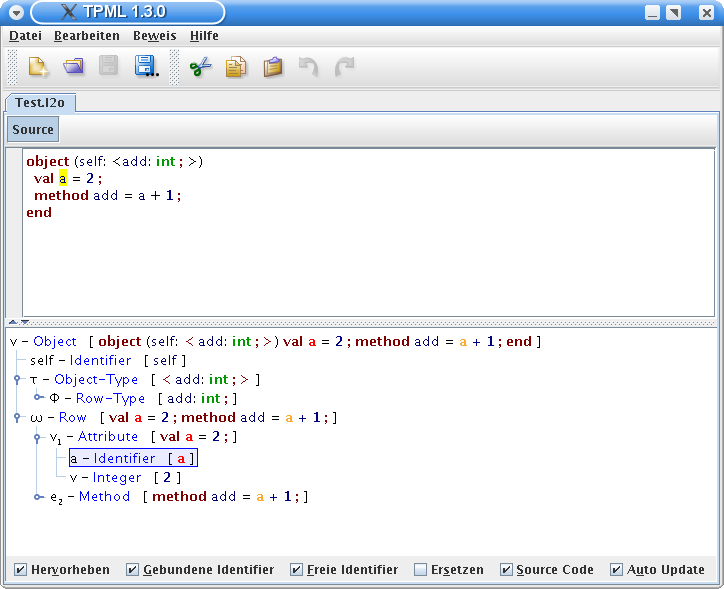
\includegraphics[width=10cm]{images/outline.png}
\caption{Outline}
\end{center}
\end{figure}

\subsection {Einstellungen}
Die Outline bietet verschiedene Einstellungsm"oglichenkeiten, die nun
kurz angesprochen werden sollen.

{\bf Hervorheben} bietet die M"oglichkeit, den aktuell in der Outline
selektierten Knoten in h"oheren Knoten zu markieren. Ist zum Beispiel
der Ausdruck \glqq$\bli{x}{\infix{+}{1}{1}}{x}$\grqq\ in der Outline geladen,
und der Knoten \glqq${\infix{+}{1}{1}}$\grqq\ selektiert, wird der zweite Ausdruck
in dem ersten hervorgehoben. Die Farbe der Hervorhebung kann, wie alle
anderen Farben auch, in den Einstellungen von \TPML\ ver"andert werden.

{\bf Gebundene} steht daf"ur, dass gebundene Identifier und Typ-Namen,
wenn sie in der Outline selektiert werden, in h"oheren Knoten 
hervorgehoben werden. Der Ausdruck \glqq$\abstr{x}{\infix{+}{x}{1}}$\grqq\ besteht
aus einen Identifier \glqq$x$\grqq\ und aus einem Kind-Ausdruck
\glqq$\infix{+}{x}{1}$\grqq. Selektiert man nun den Identifier, werden bei
aktiver Option alle Identifier hervorgehoben, die an diesen Identifier
gebunden sind. Dies funktioniert auch umgekehrt, wird also das
\glqq$x$\grqq\ im Ausdruck \glqq$\infix{+}{x}{1}$\grqq\ selektiert, wird der
Identifier hervorgehoben, an den dieser Identifier gebunden ist. Vor allem
bei komplizierteren Ausdr"ucken mit gleichen Identifiern wie 
\glqq$\bli{x}{1}{\infix{+}{x}{\bli{x}{2}{x}}}$\grqq\ k"onnen so die Bindungen
durch die Outline "uberpr"uft werden.

Wenn {\bf Freie} aktiv ist, werden freie Identifier und Typ-Namen in der
Outline hervorgehoben. Dies ist besonders n"utzlich, da freie Identifier
oder Typ-Namen meist auf eine fehlerhafte Eingabe zur"uckzuf"uhren sind.
Gibt der Anwender zum Beispiel \glqq$\bli{x}{a}{x}$\grqq\ ein, ist 
dies nat"urlich nicht falsch, aber der Type Checker w"urde den Ausdruck
nicht akzeptieren, da das \glqq$a$\grqq\ in dem Ausdruck frei 
vorkommend ist. Es werden allerdings nur Identifier und Typ-Namen
hervorgehoben, die in dem Wurzel Knoten frei vorkommend sind und nicht
alle, in den jeweiligen Knoten frei vorkommenden Identifier oder Typ-Namen.

Die Option {\bf Ersetzen} steht daf"ur, dass der selektierte Ausdruck
in h"oheren Knoten durch \glqq...\grqq\ ersetzt wird. Dadurch
werden h"ohere Knoten kompakter dargestellt, was bei gr"o"seren Ausdr"ucken
von Vorteil ist.

Ist die Option {\bf Source Code} aktiv, wird der Source Code im jeweiligen
Quelltexteditor hervorgehoben, der dem selektierten Knoten in der Outline
entspricht. Ist diese Option nicht aktiv, kann der Source Code durch einen
Doppelklick auf den Outline Knoten ebenfalls hervorgehoben werden. Diese
Option ist nur bei den Quelltexteditor verf"ugbar und nicht bei den
verschiedenen Beweiswerkzeugen.

{\bf Auto Update} steht daf"ur, dass die Outline automatisch geladen wird,
wenn sich etwas "andert, dies geschieht nach einer gewollten Verz"ogerung,
die n"otig ist, damit sich nicht zu viele "Anderungen ergeben. Diese Option
ist nur in Ansichten aktiv, in denen "Anderungen eindeutig sind, also in den
Quelltexteditoren und im Small Step Interpreter. In den anderen
Beweiswerkzeugen k"onnen bei einem Schritt mehrere Knoten erzeugt werden
und ein Laden der Outline w"are nicht eindeutig m"oglich.
Ist die Option nicht aktiv oder gar nicht verf"ugbar, kann der Anwender auf 
die entsprechenden Ausdr"ucke oder Typen klicken und diese werden dann geladen.
Gleiches gilt f"ur die Quelltexteditoren, klickt man mit der Maus auf den
Editor, wird der aktuelle Ausdruck oder Typ in die Outline geladen. Ist im
Quelltexteditor im Moment kein g"ultiger Ausdruck geladen, wird die Outline
rot umrandet.


\section {Beweiswerkzeuge}
\label{Beweiswerkzeuge} Wird ein Beweiswerkzeug gestartet, so wird
es zus"atzlich zum Quelltexteditor im Tab der Datei angezeigt. F"ur
jede Datei kann jeweils nur ein Small Step Interpreter, ein Big Step
Interpreter, ein Type Checker usw. aktiv sein. Diese k"onnen "uber die
entsprechende Schaltfl"achen angew"ahlt werden. Nat"urlich ergibt es keinen Sinn, Beweiswerkzeuge, die mit dem Typsystem zu tun haben, bei Dateien zu starten, die kein Typsystem haben, wie beispielsweise \LZERO. Wird ein
Beweiswerkzeug erneut gestartet, so ersetzt der neue Beweis ein ggf.
schon aktives Beweiswerkzeug des selben Typs. M"ochte man also zum
Beispiel einen Small Step Beweis neu starten oder f"ur einen leicht
ge"anderten Ausdruck erneut ausf"uhren, so kann dies "uber eine
erneute Anwahl der Small Step Funktion im Men"u {\bf Beweis}
geschehen. Dabei wird jedoch der aktive Small Step Interpreter durch
den neuen ersetzt.

Jedes Beweiswerkzeug verf"ugt "uber einen {\bf Beginner} und einen
{\bf Fortgeschrittener} Modus. Diese Modi unterscheiden sich in den
Regeln, zum Beweis des Ausdrucks zur Verf"ugung stehen und teilweise in der Ansicht des Beweiswerkzeuges. So werden beispielsweise beim Typ Checker im {\bf Beginner} Typen erst dann angezeigt, wenn der Typ bewiesen ist.

\subsection {Mouse-Over-Effekt}
Jeder der Beweismethoden hat f"ur den Benutzer eine weitere Komfort-Funktion eingebaut. Bei gr"o"seren Programmen, die bewiesen werden sollen, und insbesondere, wenn der gleiche Identifier doppelt benutzt wird verliert man schnell die "Ubersicht. Folgendes Beispiel soll dies verdeutlichen:

{\bf $\bli{x}{\abstr{x}{\app{x}{x}}}{\app{x}{x}}$}

Wie man leicht sieht ist der Identifier \glqq$x$\grqq\ doppelt verwendet. In noch gr"o"seren Beispielen w"are es nicht mehr einfach zu "uberschauen, an welches \glqq$x$\grqq\ welches gebunden ist. Um dies zu vereinfachen kann man einfach mit dem Mauszeiger "uber eins der \glqq$x$\grqq\ fahren, und die dazugeh"origen \glqq$x$\grqq\ werden farbig hervorgehoben. Zus"atzlich wird der Identifier, an den die anderen gebunden sind extra durch eine andere Farbe hervorgehoben\footnote{Die Farben, sowohl f"ur gebundenen als auch bindende Indentifier k"onnen "uber Einstellungen... im Men"u Bearbeiten eingestellt werden.}. Im gegebenen Beispiel w"urde das \glqq$x$\grqq\ nach dem \glqq$let$\grqq\ zusammen mit den letzten beiden \glqq$x$\grqq\ hervorgehoben, w"arend das \glqq$x$\grqq\ nach dem \glqq$lambda$\grqq\ zusammen mit den folgenden beiden \glqq$x$\grqq\ hervorgehoben w"urden.
Idetifier, die keine Bindungen haben, aber Bindungen haben k"onnten werden ebenfalls hervorgehoben. Anders Identifier, die gar keine Bindungen haben k"onnen, wie es bei Namen f"ur Methoden der Fall ist. Dazu sei ein letzte Beispiel zu diesem Thema gegeben:

{\bf object (self) method inc x y = x + 1 ; end}

Dieses Beispiel hat drei Identifier: inc, x und y. x verh"alt sich wie im oberen Beispiel. Es wird zusammen mit dem gebundenen x hervorgehoben. y dagegen hat zwar keinen weiteren gebundenen Identifier, k"onnte aber einen solchen haben. Er wird alleine hervorgehoben. inc letzlich wird nicht hervorgehoben. Es ist ein Methodenname und an den kann prinzipiell nichts gebunden sein.

\section {Tutorials}
Im folgenden wird anhand von einigen Beispielen in die
Funktionsweise der einzelnen Beweiswerkzeuge eingef"uhrt. Zun"achst
"offnen wir "uber {\bf Datei} $\rightarrow$ {\bf Neu...} einen
Editor. Wie gesagt ist jeder Editor fest mit einer Sprache
verkn"upft.

\begin{figure}[h]
\begin{center}
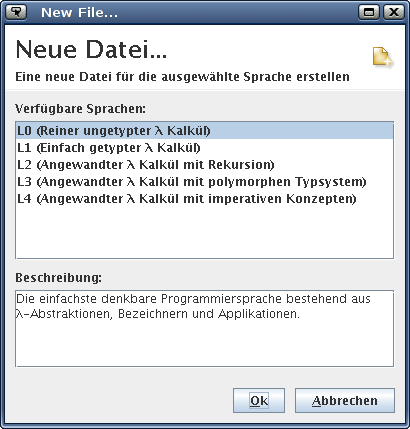
\includegraphics[width=8cm]{images/new-dialog.png}
\caption{Eine neue Datei erstellen}
\end{center}
\end{figure}

Wir w"ahlen f"ur unser Beispiel die Sprache \LONE\ aus und best"atigen
mit {\bf Ok}. Es ist nun standardm"a"sig der Quelltexteditor aktiv.
Wir geben einen Ausdruck ein, mit dem wir nun arbeiten wollen:

{\bf (lambda x.x * 3) 4}

Mit ein wenig Vorstellungskraft erkennt man, dass dieser Ausdruck
vorraussichtlich das Produkt aus 3 und 4 berechnet.


\subsection{Small Step Interpreter}
Unsere mutige Behauptung wollen wir nun nat"urlich durch einen
stichhaltigen Beweis untermauern. Wir starten also mittels {\bf
Beweis} $\rightarrow$ {\bf Small Step} oder mit der Taste F9 einen
Small Step Interpreter.

\begin{figure}[h]
\begin{center}
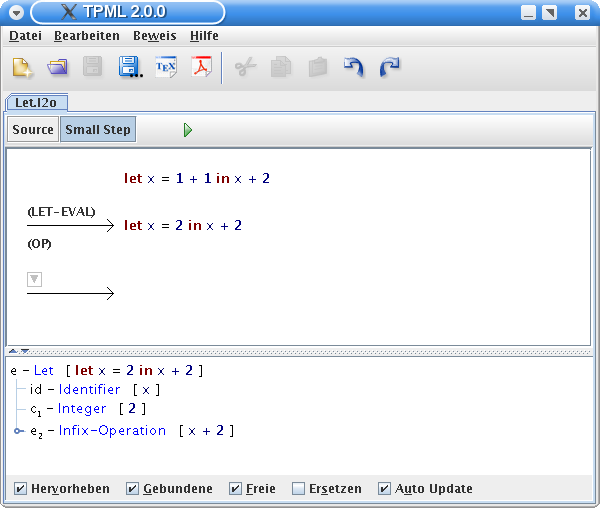
\includegraphics[width=10cm]{images/small-step.png}
\caption{Der Small Step Interpreter}
\label{FigureSmallStep}
\end{center}
\end{figure}

Bewegt man nun den Mauscursor "uber den Buttons des Regelmen"us
oberhalb des Pfeils f"ur den ersten Ableitungsschritt wird der Teil
des Ausdrucks rot unterstrichen, der als n"achstes Abgeleitet werden
soll, wie in Abbildung~\ref{FigureSmallStep} gezeigt.
In unserem Falle ist dies der gesamte Ausdruck. Der n"achste
Ableitungsschritt muss {\bf BETA-V} sein, um die 4 f"ur das x zu
substituieren. Wir klicken also auf den Button und w"ahlen in dem
erscheinenden Regelmen"u den entsprechenden Eintrag aus. Alternativ
kann man auch einzelne Schritte oder den kompletten Beweis
automatisch ausf"uhren lassen. F"ur einzelne Schritte klickt man
entweder auf den gr"unen Pfeil oberhalb des Small Step Interpreters
oder w"ahlt {\bf Raten} im Regelmen"u. Eine komplette Beweisf"uhrung
wird mittels {\bf Vervollst"andigen} im selben Men"u vorgenommen.

Ist man mit den Regeln vertraut, so kann man "uber {\bf Beweis}
$\rightarrow$ {\bf Fortgeschrittener} einige Regeln ausblenden. Das
Regelmen"u enth"alt nun nur noch Regeln die spezifizieren was getan
werden soll und nicht mehr genau wo. So muss zum Beispiel eine
Bedingung nicht mehr mit {\bf COND-EVAL} ausgewertet werden. Man
gibt w"ahlt lediglich {\bf COND-TRUE} bzw. {\bf COND-FALSE} aus.

\subsection{Big Step Interpreter}
Der Big Step Interpreter kann auch "uber das {\bf Beweis} Men"u oder
mit der Taste F11 gestartet werden. Zu beachten ist, dass man sich
hierf"ur nicht zwingend im Quelltexteditor befinden muss. Auch beim
Big Step Interpreter k"onnen Regeln "uber das Regelmen"u ausgew"ahlt
werden. Ist ein Unterbaum vollst"andig ausgewertet, so wird das
ermittelte Ergebnis f"ur h"ohere Knoten "ubernommen. Da unser
Beispiel lediglich einen Unterbaum f"ur die Regel {\bf BETA-VALUE}
enth"alt, ist dies auch gleichzeitig unser Ergebnis. Im Gegensatz
zum Small Step Interpreter gibt es aufgrund der Baumstruktur des
Beweises mehrere Stellen an denen Regeln angewandt werden k"onnen.
Die Raten-Funktion bezieht sich dabei immer auf den obersten, noch
nicht komplett ausgewerteten Teilbaum. Mit {\bf Vervollst"andigen}
wird stets nur der jeweilige Unterbaum komplett ausgewertet und
nicht wie beim Small Step Interpreter der komplette Beweis zu ende
gef"uhrt.

\subsection{Type Checker}

Diese Beweisart ist genau wie der Big Step Interpreter in einer
Baumstruktur aufgebaut. Der Type Checker verh"alt sich daher
bez"uglich des Anwenden von Regeln, den Raten und der
Vervollst"andigen Funktion genau wie der Big Step Interpreter. Das
Anf"ugen von Typvariablen geschieht bei Regelanwendung automatisch.

Alternativ kann man mit der Funktion {\bf Typ eingeben} in dem
Regelmen"u selbst einen Typ f"ur den entsprechenden Teilbaum
eingeben, wie in Abbildung~\ref{FigureTypeChecker} gezeigt.
Der Typinferenzalgorithmus versucht dann den Unterbaum zu
diesem Typ auszuwerten.

\begin{figure}[h]
\begin{center}
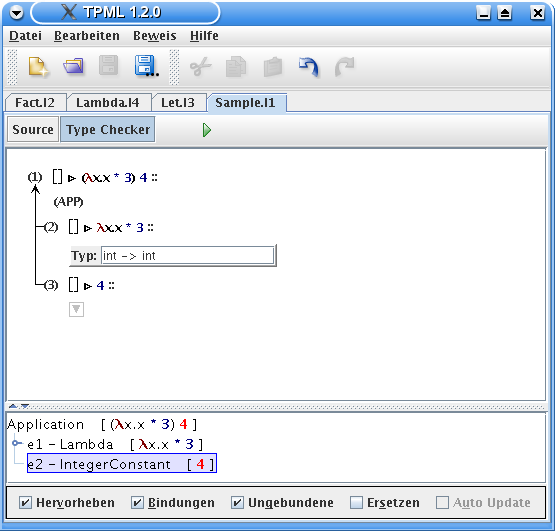
\includegraphics[width=10cm]{images/type-checker.png}
\caption{Der Type Checker}
\label{FigureTypeChecker}
\end{center}
\end{figure}

\subsection{Type Inference}
Der Type Inference Algorithmus ist, wie der Small Step Interpreter 
auch, in einer Listenstruktur realisiert, und kann "uber {\bf Beweis} 
$\rightarrow$ {\bf Type Inference} gestartet werden. Die Bedienung ist auch diesmal 
wieder an die bereits genannten Beweisarten angelehnt. Es besteht 
auch hier die M"oglichkeit selber Regeln auf den aktuellen Ausdruck
anzuwenden, den n"achsten Schritt erraten zu lassen, oder den kompletten
Ausdruck zu vervollst"andigen.

Wendet man die Regel Unify an, werden die evtl. daraus hervorgehenden
Type Substitutions in einer Liste "uber den Type Formulas gesammelt. 
Dabei ist die zuletzt gesammelte Type Substitution sichtbar. Die bereits
vorher gesammelten Type Substitutions werden durch drei Punkte angedeutet,
und k"onnen als Tooltip "uber den Punkten eingesehen werden.

Wenn man sich etwas mit der Funktionsweise des Algorithmus vertraut gemacht hat,
kann man "uber {\bf Beweis} $\rightarrow$ {\bf Fortgeschrittener} in den 
Advanced Modus wechseln. In diesem Modus werden Type Equations, bei denen beide
Typvariablen aus Arrow Types bestehen, jetzt nicht mehr neue Type Equations
aufgenommen, sondern diese werden direkt zu Type Substitutions aufgel"ost.
Ausserdem wird beim Anwenden einer Regel auf den Ausdruck nicht mehr vom System
versucht die Regel einer Type Formula zuzuordnen, sondern es wird versucht die Regel
auf die erste Type Formula anzuwenden. Diese k"onnen allerdings durch Drag 
and Drop umsortiert werden.

Das Regelwerk ist, mit einer Ausnahme, "aquivalent zum Type Checker. Es wurde 
noch die Regel {\bf UNIFY} hinzugenommen. Die sich aus folgenden Ableitungsschritten
zusammensetzt:\\[4mm] 

\begin{tabular}{ll}
  (EMPTY)\    & $\unify(A,\emp) = [\,]$ \\[3mm]
  (ASSUME)\   & $\unify(A,\{\tau = \tau'\} \cup E) = \unify(A,E) \mbox{  falls } (\tau = \tau') \in A $\\[3mm]
  (TRIV)\     & $\unify(A,\{\tau = \tau\} \cup E) = \unify(A,E)$\\[3mm]
  (MU-LEFT)\  & $\unify(A,\{\rectype{t}{\tau} = \tau'\} \cup E) = 
                 \unify(A,\{\tau [\rectype{t}{\tau}/t] = \tau'\} \cup E)$\\[3mm]
  (MU-RIGHT)\ & $\unify(A,\{\tau = \rectype{t}{\tau'}\} \cup E) = 
                 \unify(A,\{\tau = \tau' [\rectype{t}{\tau'}/t]\} \cup E)$\\[3mm]
  (VAR)\      & $\unify(A,\{\alpha = \tau\} \cup E) = \unify(A,\{\tau = \alpha\} \cup E)$\\[2mm]
              & $\ =\, \bcase 
                        [\tau/\alpha] \circ s & 
                        \mbox{falls } \alpha \notin \var{\tau} \mbox{ und } 
                        \unify(E[\tau/\alpha]) = s \\[2mm]
                        \fail         & \mbox{falls } \alpha \notin \var{\tau} \mbox{ und }\\&
                        \unify(E[\tau/\alpha]) = \fail\\[1mm]
                        & \mbox{oder } \alpha \in \var{\tau} \mbox{ und } \alpha \neq \tau
                        \ecase\vspace{3mm}$\\
  (ARROW)\    & $\unify(A,\{\tau_1 \to \tau_2 = \tau'_1 \to \tau'_2\} \cup E)$\\[1mm]
              & \quad $= \unify(A \cup \{\tau_1 \to \tau_2 = \tau'_1 \to \tau'_2\},
                \{\tau_1 = \tau'_1,\,\tau_2 = \tau'_2\} \cup E)$\\[3mm]
  (TUPLE)\    & $\unify(A,\{\tau_1 *\ \ldots\ * \tau_n = \tau_1' *\ \ldots\ * \tau_n'\} \cup E)$\\[1mm]
              & \quad $= \unify(A \cup \{\tau_1 *\ \ldots\ * \tau_n = \tau_1' *\ \ldots\ * \tau_n'\},$\\
              & \quad \quad $\{\tau_1 = \tau_1',\ \ldots\ , \tau_n = \tau_n'\} \cup E)$\\[3mm]
  (LIST)\     & $\unify(A,\{\listtype{\tau} = \listtype{\tau'} \} \cup E)$\\[1mm]
              & \quad $= \unify(A \cup \{\listtype{\tau} = \listtype{\tau'} \},
                         \{\tau = \tau' \} \cup E)$\\[3mm]
  (REF)\      & $\unify(A,\{\reftype{\tau} = \reftype{\tau'} \} \cup E)$\\[1mm]
              & \quad $= \unify(A \cup \{\reftype{\tau} = \reftype{\tau'} \},
                         \{\tau = \tau' \} \cup E)$\\[3mm]
  (OBJECT)\   & $\unify(A,\{\objecttype{\phi}\ =\ \objecttype{\phi'} \} \cup E)$\\[1mm]
              & \quad $= \unify(A \cup \{\objecttype{\phi}\ =\ \objecttype{\phi'} \},
                         \{\phi = \phi' \} \cup E)$\\[3mm]
  (ROW)\      & $\unify(A,\{ (m_1 = \tau_1\ ;\ \ldots\ ;\ m_n = \tau_n;\ \phi)$\\
              & \quad $= (m_1 = \tau_1'\ ;\ \ldots\ ;\ m_n = \tau_n';\ \phi') \} \cup E)$\\[1mm]
              & \quad $= \unify(A \cup \{ (m_1 = \tau_1\ ;\ \ldots\ ;\ m_n = \tau_n;\ \phi)$\\
              & \quad \quad $= (m_1 = \tau_1'\ ;\ \ldots\ ;\ m_n = \tau_n';\ \phi') \},$\\
              & \quad \quad \quad $\{\tau_1 = \tau_1', \ \ldots\ ,\tau_n = \tau_n',
                \phi = \phi' \} \cup E)$\\[3mm]
  (STRUCT)\   & $\unify(A,\{\tau_1 = \tau_2\} \cup E) = \fail$\\[1mm]
              & in  allen anderen F\"allen
\end{tabular}\\[6mm]
Bei der Regel {\bf ROW} ist darauf zu achten, dass die Methodennamen nicht in der gleichen Reihenfolge
vorkommen m"ussen. Ebenfalls m"ussen die Methodennamen nicht in beiden Reihen vorkommen, da f"ur den Fall, 
dass $\phi$ nicht gleich $\epsilon$ ist, $\unify$ auch mit $\phi$ und den restlichen Methoden von $\tau'$ 
aufgerufen werden kann. Zum Beispiel f"uhrt $\unify (A,\{ (b: \alpha_1 ; \alpha_2) = (a: int ; b: int ;)\}
\cup E)$ zu dem Aufruf von $\unify (A \cup \{ (b: \alpha_1 ; \alpha_2) = (a: int ; b: int ;)\},
\{\alpha_1 = int, \alpha_2 = a: int\} \cup E)$.

\subsection{Minimal Typing}
Der Minimal Typing Algorithmus ist, wie der Big Stepper und der Type Checker, in einer Baumstruktur realisiert.
Auch die Bedienung dieser Beweismethode ist "aquivalent zu den beiden anderen. Es besteht auch hier die M"oglichkeit
die n"achste Regel "uber das Pull Down Men"u auszuw"ahlen, einen Schritt vom Algorithmus selbst erraten zu lassen,
oder den kompletten Beweis vervollst"andigen zu lassen. F"ur den Fall, dass der Ausdruck synktaktischen Zucker 
enth"alt, kann auch hier in Kernsyntax "ubersetzt werden.

\subsection{Sub Typing}
Zur "Uberpr"ufung von Subtyprelationen wurde ein eigener Source Editor angelegt. Dieser beinhaltet zwei Eingabefelder,
welche von Bedienung und Aussehen dem normalen Source Editor gleichen, allerdings nur f"ur die Eingabe von Typen gedacht
sind, und nicht f"ur ganze Expressions. Das erste Eingabefeld soll den Subtyp entgegennehmen, und das zweite Eingabefeld 
den Supertyp, fu"r welche man die Subtyp Realation "uberpr"ufen will. Ein weiterer Unterschied zum allgemeinen Source 
Editor ist, dass man eine Outline pro Eingabefeld hat, statt wie vorher insgesamt eine Outline.

F"ur den Beweis hat man die Wahl zwischen einfachem Sub Typing, und Sub Typing mit rekursiven Typen. Beide sind von 
Bedienung und Aussehen her exakt gleich. Auch hier wurde bei der Visualisierung wieder eine Baumstruktur verwendet,
und von die Bedienung gleicht Subtyping den schon bekannten Beweismethoden. 



% vi:set syntax=tex ts=2 sw=2 et encoding=UTF-8:
